%%%%%%%%%%%%%%%%%%%%%%%%%%%%%%%%%%%%%%%%%
% Template ini dibuat untuk makalah kolokium mahasiswa
% Program Alih Jenis (Ekstensi) Ilmu Komputer IPB
% Version 1.0 (18/05/2015)
%
% Template ini menggunakan template yang di-download dari:
% http://www.LaTeXTemplates.com
% Mathias Legrand (legrand.mathias@gmail.com)
% License: CC BY-NC-SA 3.0 (http://creativecommons.org/licenses/by-nc-sa/3.0/)
%
% Dimodifikasi untuk keperluan Program Studi
% Oleh: JULIO ADISANTOSO (julioipb@gmail.com)
%
% Untuk memudahkan penggunaan, maka diambil contoh makalah atas nama 
% Fithranto Faturakhman di bawah bimbingan Karlisa Priandana ILKOM-IPB.
% Silakan mengganti dan melengkapi file:
%    (1) kolokium_information.tex -- judul, nama, nim, email, pembimbing, dsb
%    (2) abstrak.tex -- abstrak makalah
%    (3) pendahuluan.tex -- berisi latar belakang, dsb
%    (4) metode.tex -- berisi metode penelitian
%    (5) daftar_pustaka.tex -- berisi daftar pustaka
%
%%%%%%%%%%%%%%%%%%%%%%%%%%%%%%%%%%%%%%%%%

%----------------------------------------------------------------------------------------
%	PACKAGES AND OTHER DOCUMENT CONFIGURATIONS
%----------------------------------------------------------------------------------------

\documentclass[fleqn,11pt]{SelfArx} % Document font size and equations flushed left
\usepackage[english]{babel}

%----------------------------------------------------------------------------------------
%	COLUMNS
%----------------------------------------------------------------------------------------

\setlength{\columnsep}{0.55cm} % Distance between the two columns of text
\setlength{\fboxrule}{0.75pt} % Width of the border around the abstract

%----------------------------------------------------------------------------------------
%	COLORS
%----------------------------------------------------------------------------------------

\definecolor{color1}{RGB}{0,0,90} % Color of the article title and sections
\definecolor{color2}{RGB}{0,20,20} % Color of the boxes behind the abstract and headings

%----------------------------------------------------------------------------------------
%	HYPERLINKS
%----------------------------------------------------------------------------------------

\usepackage{hyperref} % Required for hyperlinks
\hypersetup{hidelinks,colorlinks,breaklinks=true,urlcolor=color2,citecolor=color1,linkcolor=color1,bookmarksopen=false,pdftitle={Title},pdfauthor={Author}}


%
% Hyphenation untuk Indonesia 
%
% @author  Andreas Febrian
% @version 1.00
% 
% Tambahkan cara pemenggalan kata-kata yang salah dipenggal secara otomatis 
% oleh LaTeX. Jika kata tersebut dapat dipenggal dengan benar, maka tidak 
% perlu ditambahkan dalam berkas ini. Tanda pemenggalan kata menggunakan 
% tanda '-'; contoh: menarik  --> pemenggalan: me-na-rik
%

\hyphenation{
    % alphabhet A
    a-na-li-sa a-tur 
    a-pli-ka-si 
    % alphabhet B
    ba-ngun-an 
    be-be-ra-pa 
    ber-ge-rak
    ber-ke-lan-jut-an 
    ber-pe-nga-ruh 
    Bha-dri-ra-ju
    % alphabhet C
    ca-ri
    % alphabhet D
    di-sim-pan di-pim-pin de-ngan da-e-rah di-ba-ngun da-pat di-nya-ta-kan 
    di-sim-bol-kan di-pi-lih di-li-hat de-fi-ni-si
    % alphabhet E
    e-ner-gi eks-klu-sif
    % alphabhet F
    fa-si-li-tas
    % alphabhet G
    ga-bung-an ge-rak
    % alphabhet H
    ha-lang-an
    % alphabhet I
    % alphabhet J
    jang-krik
    % alphabhet K
    ke-hi-lang-an
    ku-ning 
    kua-li-tas ka-me-ra ke-mung-kin-an ke-se-pa-ham-an
    % alphabhet L
    ling-kung-an
    % alphabhet M
    me-neng-ah
    meng-a-tas-i me-mung-kin-kan me-nge-na-i me-ngi-rim-kan 
    meng-u-bah meng-a-dap-ta-si me-nya-ta-kan mo-di-fi-ka-si
    meng-a-tur meng-um-pul-kan Men-te-ri
    Mo-ham-med
    % alphabhet N
    nya-ta non-eks-klu-sif
    % alphabhet O
    % alphabhet P
	pe-nye-rap-an 
	pe-ngon-trol
    pe-mo-del-an
    pe-ran  pe-ran-an-nya
    pem-ba-ngun-an pre-si-den pe-me-rin-tah prio-ri-tas peng-am-bil-an 
    peng-ga-bung-an pe-nga-was-an pe-ngem-bang-an 
    pe-nga-ruh pa-ra-lel-is-me per-hi-tung-an per-ma-sa-lah-an 
    pen-ca-ri-an peng-struk-tur-an
    PER-TAM-BANG-AN
    % alphabhet Q
    % alphabhet R
    ran-cang-an
    % alphabhet S
    si-mu-la-si sa-ngat Sa-ma-rin-da
    % alphabhet T
    te-ngah
    ter-da-pat
    % alphabhet U
    % alphabhet V
    % alphabhet W
    % alphabhet X
    % alphabhet Y
    % alphabhet Z
    % special
}
% Tuliskan nama lengkap Anda
\def\namaMhs {Bayu Santoso}

% Tuliskan NIM Anda
\def\nim {G64134017}

% Tuliskan alamat email Anda
\def\emailMhs {bayusantoso.mail@gmail.com}

% Tuliskan nama lengkap dosen pembimbing
\def\namaDosen {Yeni Herdiyeni}

% Tuliskan judul makalah kolokium di definisi "judul"
\def\judul {Pembangunan \textit{Biodiversity Informatics} Genetika Tumbuhan Obat Berbasis Ontologi}

% Tuliskan kata kunci, dipisahkan oleh tanda titik-koma
\def\katakunci {\textit{biodiversity informatics}; tumbuhan obat; ontologi; web semantik}


\usepackage{xcolor,colortbl}
\usepackage{multicol}
\usepackage{multirow}
\usepackage[urldate=iso8601, backend=biber, style=authoryear, url=true, doi=true, sorting=nyt]{biblatex}
\addbibresource{pustaka.bib}
\DefineBibliographyStrings{english}{%
	urlseen = {diunduh pada},
}
\renewbibmacro{in:}{\xspace dalam:}
\renewbibmacro*{volume+number+eid}{%
	\printfield{volume}%
	%  \setunit*{\adddot}% DELETED
	\setunit*{\addnbspace}% NEW (optional); there's also \addnbthinspace
	\printfield{number}%
	\setunit{\addcomma\space}%
	\printfield{eid}}
\DeclareFieldFormat[article]{number}{\mkbibparens{#1}}

%----------------------------------------------------------------------------------------
%	ARTICLE INFORMATION
%----------------------------------------------------------------------------------------

\JournalInfo{Makalah Kolokium Program S1 Ilmu Komputer Alih Jenis} % Journal information
\Archive{Departemen Ilmu Komputer, FMIPA-IPB} % Departemen ILKOM-IPB

\PaperTitle{\judul} 

\Authors{\namaMhs (\nim)*, \namaDosen} % Penulis
\affiliation{*\scriptsize\textbf{Alamat Email}: \emailMhs \normalsize} % Corresponding author

\Keywords{\scriptsize \katakunci \normalsize} 
\newcommand{\keywordname}{Kata Kunci} % Defines the keywords heading name

%----------------------------------------------------------------------------------------
%	ABSTRACT
%----------------------------------------------------------------------------------------
\Abstract{\scriptsize 
% ---- Tuliskan abstrak di bagian ini seperti contoh.
Indonesia memiliki lebih dari 32.000 spesies tumbuhan. Dari kumpulan spesies tersebut terdapat tumbuhan obat di dalamnya. Tidak kurang dari 2039 spesies tumbuhan obat berasal dari hutan Indonesia. Saat ini hutan Indonesia mengalami kerusakan dan kepunahan. Oleh karena itu, diperlukan upaya untuk melestarikan tumbuhan obat. Salah satu cara untuk melestarikan tumbuhan obat adalah dengan cara mengenali tumbuhan obat.  Informasi yang dibutuhkan mengenai tumbuhan obat sulit untuk ditemukan.  Berdasarkan hal tersebut maka muncul bidang baru dalam pengumpulan informasi tumbuhan yang bernama \textit{biodiversity informatics}. Metode pemodelan data yang dapat menangani sistem berbasis inferensi adalah ontologi. Ontologi dapat diterapkan pada web semantik. Penelitian ini akan mengembangkan sistem web semantik yang memberikan informasi genetika tumbuhan obat. Selain itu sistem web semantik ini akan menyediakan \textit{web service} yang memungkinkan untuk terintegrasi dengan sistem web semantik yang lain.
% ---- Akhir bagian abstrak
\normalsize}


%----------------------------------------------------------------------------------------

\begin{document}

\flushbottom % Makes all text pages the same height

\maketitle % Print the title and abstract box

\thispagestyle{empty} % Removes page numbering from the first page

%----------------------------------------------------------------------------------------
%	BAGIAN PENDAHULUAN
%----------------------------------------------------------------------------------------

%----------------------------------------------------------------------------------------
%	PENDAHULUAN
%----------------------------------------------------------------------------------------
\section*{PENDAHULUAN} % Sub Judul PENDAHULUAN
% Tuliskan isi Pendahuluan di bagian bawah ini. 
% Jika ingin menambahkan Sub-Sub Judul lainnya, silakan melihat contoh yang ada.
% Sub-sub Judul 
\subsection*{Latar Belakang}
Indonesia memiliki lebih dari 32.000 spesies tumbuhan (\citeauthor{BAPPENAS2003} \cite*{BAPPENAS2003}). Dari kumpulan spesies tersebut terdapat tumbuhan obat di dalamnya. Menurut \citeauthor{ZUHUD2008} (\cite*{ZUHUD2008}) tidak kurang dari 2039 spesies tumbuhan obat berasal dari hutan Indonesia. Tanaman obat yang beraneka ragam jenis, habitus, dan khasiatnya mempunyai peluang besar serta memberi kontribusi bagi pembangunan dan pengembangan hutan (\citeauthor{HAMZARI2008} \cite*{HAMZARI2008}). Saat ini hutan Indonesia mengalami kerusakan dan kepunahan (\citeauthor{ZUHUD2008} \cite*{ZUHUD2008}). Oleh karena itu, diperlukan upaya untuk melestarikan tumbuhan obat. Salah satu cara untuk melestarikan tumbuhan obat adalah dengan cara mengenali tumbuhan obat (\citeauthor{HAMZARI2008} \cite*{HAMZARI2008}). \textit{Biodiversity Informatics} merupakan upaya untuk membuat sumber informasi keanekaragaman hayati global tersedia dalam format digital yang efisien, dan untuk mengembangkan alat yang efektif dalam menganalisis dan memahami data tersebut (\citeauthor{GILLMANE2009} \cite*{GILLMANE2009}). Informasi yang dapat diperoleh dari \textit{biodiversity informatics} adalah informasi mengenai taksonomi, gambar tumbuhan, lingkungan, dan DNA tumbuhan. 

Impementasi dari \textit{biodiversity informatics} sudah menghasilkan beberapa sistem yang menyediakan informasi mengenai tumbuhan.  Integrated Taxonomic Information System  (ITIS) dan Global Biodiversity Information Facility (GBIF) menyediakan informasi yang luas tentang tumbuhan. Sistem tersebut dibuat dengan menggunakan model basis data relasional. Model basis data relasional menimbulkan masalah apabila digunakan pada sistem berbasis inferensi (\citeauthor{LAALLAM2013} \cite*{LAALLAM2013}). Selain itu model basis data relasional dapat menghasilkan data yang berganda. Oleh sebab itu, dibutuhkan pemodelan data yang dapat mengatasi hal tersebut. Metode pemodelan data yang dapat menangani sistem berbasis inferensi adalah ontologi.

Ontologi adalah metode yang digunakan untuk merepresentasikan ide, fakta dan lain sebagainya, yang digunakan untuk mendefinisikan hubungan dan klasifikasi dari pengetahuan tertentu (\citeauthor{JEPSEN2010} \cite*{JEPSEN2010}). Ontologi dapat menentukan kelas, hubungan, fungsi dan objek lain (\citeauthor{DILECCE2008} \cite*{DILECCE2008}). Selain itu, model ontologi lebih sesuai diterapkan pada web semantik dibandingkan dengan model basis data relasional (\citeauthor{LAALLAM2013} \cite*{LAALLAM2013}).

Penelitian dengan menggunakan ontologi mengenai tumbuhan obat sudah banyak dilakukan, seperti penelitian tentang ontologi yang digunakan untuk menganalisis hubungan tumbuhan obat dengan istilah medis yang standar (\citeauthor{VADIVU2012} \cite*{VADIVU2012}). Penelitian yang terkait dengan ontologi gen juga sudah pernah dilakukan untuk menghasilkan data gen yang dinamis dan terkontrol (\citeauthor{ASHBURNERM2000} \cite*{ASHBURNERM2000}). Namun, penelitian tersebut belum menghasilkan hubungan antara tumbuhan obat dengan infomasi gen-nya. Pada penelitian ini akan dibuat sistem yang memanfaatkan web semantik yang digunakan untuk mengintegrasikan informasi gen dengan tumbuhan obat. \textit{Resource Description Framework} (RDF) akan diterapkan pada sistem ini untuk mengatasi masalah integrasi dengan data tumbuhan obat. RDF merupakan standar untuk merepresentasikan data yang berbentuk grafik dan membagikan dengan manusia dan mesin. 

Berdasarkan latar belakang di atas penelitian ini akan mengembangkan sistem web semantik yang memberikan informasi gen tumbuhan obat. Selain itu sistem web semantik ini akan menyediakan \textit{web service} yang memungkinkan untuk terintegrasi dengan sistem web semantik yang lain.

% Sub-sub Judul 
\subsection*{Tujuan}
Tujuan yang ingin dicapai dalam penelitian ini adalah:
\begin{enumerate}[noitemsep] 
\item Menerapkan teknologi web semantik untuk menggunakan ontologi gen (\textit{gene ontology}).
\item Mengintegrasikan sistem ontologi gen dengan data tumbuhan obat.
\item Mengintegrasikan sistem ontologi gen dengan sistem yang lain, yaitu ontologi tumbuhan (\textit{plant ontology}) dan ontologi lingkungan (\textit{environment ontoloy}).
\end{enumerate}

\subsection*{Ruang Lingkup}
Ruang lingkup penelitian adalah:
\begin{enumerate}[noitemsep] 
\item Ontologi yang digunakan dalam penelitian ini berasal dari situs geneontology.org.
\item Data korpus yang digunakan terbatas hanya tumbuhan obat. 
\item Sistem ontologi gen yang dibangun diintegrasikan dengan ontologi tanaman dan ontologi lingkungan.
\end{enumerate}

\subsection*{Manfaat}
Hasil pengembangan sistem ontologi gen ini diharapkan dapat membantu memberikan informasi mengenai gen dari tumbuhan obat.


%----------------------------------------------------------------------------------------
%	BAGIAN METODE
%----------------------------------------------------------------------------------------

%----------------------------------------------------------------------------------------
%	METODE
%----------------------------------------------------------------------------------------
\section*{METODE PENELITIAN}

\subsection*{Data Penelitian}

Data yang digunakan pada penelitian ini ini adalah data tumbuhan obat yang diintegrasikan dengan data ontologi gen yang berasal dari situs geneontology.org.

\subsection*{Tahapan Penelitian}

Tahapan-tahapan yang dilakukan pada penelitian ini mengacu pada metode pengembangan aplikasi SW-OODM. Tahapan pengembangan aplikasi SW-OODM dapat dilihat pada Gambar \ref{fig:tahapan_penelitian}.

\begin{figure}[h!] % Gunakan \begin{figure*} untuk memasukkan Gambar
	\centering
	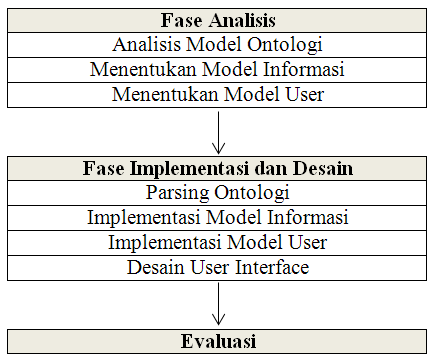
\includegraphics[width=200pt]{kolokium_tahapan_penelitian_gb2.png}
	\caption{Tahapan Penelitian}
	\label{fig:tahapan_penelitian}
\end{figure}

Fase Analisa
Pada fase analisa terdapat 3 aktivitas yang akan dilakukan, yaitu analisis model ontologi, menentukan model informasi, menentukan model user. Aktivitas analisis model ontologi akan diidentifikasi model dari ontologi gen. Hasil identifikasi model ontologi digambarkan dengan bentuk graph, sehingga bentuk dari ontologi gen akan dapat lebih mudah dipelajari.

Aktivitas menentukan model informasi akan memanfaatkan hasil dari analisis model ontologi untuk menentukan kelas, atribut dan keterkaitan antar objek yang ada di dalam ontologi. Pada aktivitas menentukan model user akan didefinisikan diagram use case, class diagram, activitiy diagram dan sequence diagram.

Fase Implementasi dan Desain

Pada fase implementasi dan desain akan diawali dengan parsing ontologi. Hasil dari parsing ontologi dapat digunakan untuk template ontologi, sehingga dari template tersebut mesin dapat memahami model dari ontologi gen. Pada tahapan implementasi model akan dihasilkan fungsi-fungsi dari sistem ontologi gen yang berupa web. Pada tahapan implementasi user akan menghasilkan fungsi yang dapat digunakan oleh pengguna agar dapat berinteraksi dengan sistem. Tahap desain \textit{user interface} akan menghasilkan halaman desain halaman yang diakses pengguna yang dapat memudahkan pengguna dalam menggunakan sistem.

Evaluasi

Fase evaluasi akan dilakukan pengujian dari sistem yang sudah dibuat. Pengujian yang dilakukan meliputi kecepatan proses pencarian dari sistem yang dibuat, kelengkapan data yang dihasilkan dari proses pencarian, dan kecocokan hasil pencarian dengan kata kunci pencarian.


\subsection*{Lingkungan Pengembangan}

Pembangunan sistem ontologi gen tanaman obat berbasis web ini dilakukan dengan menggunakan perangkat keras dan perangkat lunak sebagai berikut:

\begin{itemize}
	\item Prosesor Intel Core i7 4500U 1,8 GHz
	\item Memori 12 GB
	\item Hard disk 1 TB
	\item Sistem operasi Windows 7 Ultimate
	\item Bahasa pemrograman Python dengan Flask sebagai web framework
	\item RDFLib sebagai library yang digunakan untuk penggunaan RDF pada Phyton
	\item Lingkungan pengembangan (IDE) Visual Studio 2013 
	\item Protégé 4.3.0 sebagai pemodelan ontologi
\end{itemize}

\subsection*{Rencana Jadwal Penelitian}

\begin{table*}[h!]
	\begin{center}
		\caption{Rencana Jadwal Penelitian}
		\label{tab:jadwal}
		\footnotesize
		\begin{tabular}{|l|c|c|c|c|c|c|c|c|c|c|c|c|c|c|c|c|c|c|c|c|c|c|c|c|}
			\hline
			\multirow{2}{*}{Kegiatan}&\multicolumn{2}{c|}{Mei}&\multicolumn{4}{c|}{Juni}&\multicolumn{4}{c|}{Juli}&\multicolumn{4}{c|}{Agustus}&\multicolumn{4}{c|}{September}&\multicolumn{4}{c|}{Oktober}&\multicolumn{2}{c|}{November}\\
			\cline{2-25}
			&3&4&1&2&3&4&1&2&3&4&1&2&3&4&1&2&3&4&1&2&3&4&1&2\\
			\hline
			Penyusunan Proposal Skripsi&\cellcolor{black}&\cellcolor{black}&\cellcolor{black}&\cellcolor{black}&\cellcolor{black}&&&&&&&&&&&&&&&&&&&\\
			\hline
			Kolokium&&&&&&\cellcolor{black}&&&&&&&&&&&&&&&&&&\\
			\hline
			Pengumpulan Data&\cellcolor{black}&\cellcolor{black}&\cellcolor{black}&\cellcolor{black}&\cellcolor{black}&\cellcolor{black}&&&&&&&&&&&&&&&&&&\\
			\hline
			Fase Analisis&&&&&&&\cellcolor{black}&\cellcolor{black}&&&&&&&&&&&&&&&&\\
			\hline
			Fase Implementasi data&&&&&&&&&\cellcolor{black}&\cellcolor{black}&\cellcolor{black}&\cellcolor{black}&\cellcolor{black}&\cellcolor{black}&\cellcolor{black}&\cellcolor{black}&&&&&&&&\\
			\hline
			Fase Evaluasi&&&&&&&&&&&&&&&&&\cellcolor{black}&\cellcolor{black}&&&&&&\\
			\hline
			Penulisan Skripsi&&&&&&&&&\cellcolor{black}&\cellcolor{black}&\cellcolor{black}&\cellcolor{black}&\cellcolor{black}&\cellcolor{black}&\cellcolor{black}&\cellcolor{black}&\cellcolor{black}&\cellcolor{black}&\cellcolor{black}&&&&&\\
			\hline
			Seminar&&&&&&&&&&&&&&&&&&&&\cellcolor{black}&&&&\\
			\hline
			Sidang skripsi&&&&&&&&&&&&&&&&&&&&&&\cellcolor{black}&&\\
			\hline
			Perbaikan laporan penelitian&&&&&&&&&&&&&&&&&&&&&&&\cellcolor{black}&\cellcolor{black}\\
			\hline
		\end{tabular}
		\normalsize
	\end{center}
\end{table*}

%----------------------------------------------------------------------------------------
%	BAGIAN DAFTAR PUSTAKA
%----------------------------------------------------------------------------------------

\renewcommand{\refname}{DAFTAR PUSTAKA}
\nocite{*}
\printbibliography

%----------------------------------------------------------------------------------------

\end{document}